\section{Steady response}\label{sec:resonance}
Substituting $x = \operatorname{Re}\bigl(\hat x\,e^{i\Omega t}\bigr)$ into \cref{eq:normal} and
writing $r = \Omega/\wn$ gives
\begin{equation}\label{eq:amp}
  \frac{\abs{\hat x}}{F_0/k} = \frac{1}{\sqrt{(1-r^2)^2 + (2\zeta r)^2}} .
\end{equation}

\begin{proposition}\label{prop:peak}
For $\zeta < 1/\sqrt{2}$ the amplitude~\eqref{eq:amp} peaks at $r = \sqrt{1-2\zeta^2}$ with height
$1/\bigl(2\zeta\sqrt{1-\zeta^2}\bigr)$.
\end{proposition}

\begin{figure}[ht]
  \centering
  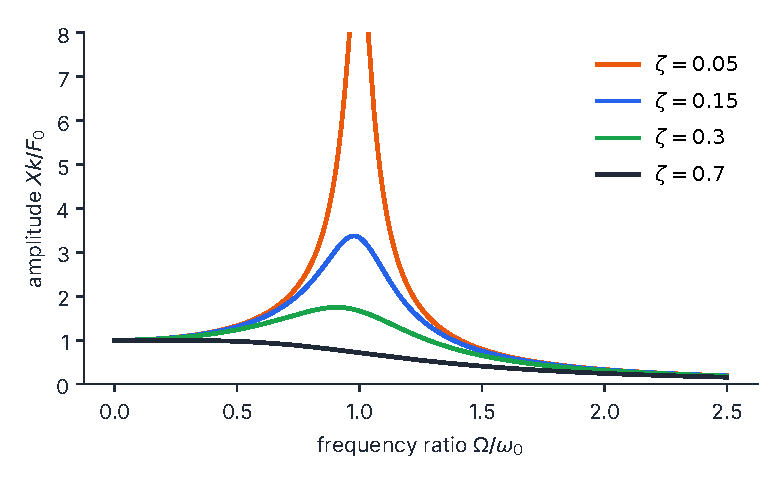
\includegraphics[width=0.75\linewidth]{figures/resonance.pdf}
  \caption{Resonance curves~\eqref{eq:amp} for four damping ratios.}
  \label{fig:resonance}
\end{figure}

\begin{table}[ht]
  \centering
  \caption{Fitted parameters (simulated data).}\label{tab:fit}
  \begin{tabular}{lrr}
    \hline
    Quantity & Value & Uncertainty \\
    \hline
    $\wn/2\pi$ & 1.62 Hz & 0.01 Hz \\
    $\zeta$ & 0.061 & 0.004 \\
    $Q = 1/(2\zeta)$ & 8.2 & 0.5 \\
    \hline
  \end{tabular}
\end{table}

The fitted values in \cref{tab:fit} give a peak height of $8.2$, in line with
\cref{prop:peak}. A quality factor this large means the oscillator selects a narrow band of
frequencies~\cite{Landau1976}.
